\documentclass{article}
\usepackage[utf8]{inputenc}
\usepackage[margin=1in,includefoot]{geometry}
\usepackage{graphicx}
\usepackage{subcaption}
\usepackage{enumerate}
\usepackage{xfrac}
\usepackage{url}
\usepackage{amsmath}
\usepackage{mathtools}
\usepackage{blindtext}
\usepackage[numbers,sort&compress]{natbib}
\usepackage{listings}
\usepackage{color}
\usepackage{filecontents}
\usepackage{natbib}
\usepackage{bibentry}
\nobibliography*
\lstset{language=Matlab,
basicstyle=\ttfamily,
keywordstyle=\color{blue}\ttfamily,
stringstyle=\color{red}\ttfamily,
commentstyle=\color{green}\ttfamily,
morecomment=[l][\color{magenta}]{\#}
}
\usepackage{multicol}
\begin{filecontents}{mytestbib.bib}
@book{goossens93,
    author = "Cambridge University Department of Engineering",
    title = "3G1 Laboratory: Investigating the lac Operon",
    year = "2017",
    publisher = "University of Cambridge",
}
@book{permease,
    author = "Crandall, M; Koch, A.L",
    title = "Temperature-Sensitive Mutants of Escherichia Coli Affecting Beta-Galactoside Transport",
    year = "1971",
    publisher = "Journal of Bacteriology. 105 (2): 609-19",
}
@book{miller,
    author = "Miller JH",
    title = "A Short Course In Bacterial Genetics: A Laboratory Manual And Handbook For Escherichia Coli And Related Bacteria",
    year = "1992",
    publisher = "Trends in Biochemical Sciences-Library Compendium, 18:193",
}
\end{filecontents}

\begin{document}
\begin{titlepage}
	\begin{center}
	\line(1,0){450}\\
	[0.25in]
	\huge{\bfseries 3G1 Investigating the lac Operon} \\
	[0.25in]
     \large Investigation on the feedback system of the lac Operon under different conditions\\
     \line(1,0){450} \\
	[12cm]
	\textsc{\Large Xiaoding Lu \\[1cm] xl402 \\ Pembroke College \\[1.2cm] 07.11.2018}\\
	\end{center}
	\begin{flushright}

	\begin{figure}[htp]
	\begin{flushright}
	\end{flushright}
	\end{figure}
	\end{flushright}

\vspace{2cm}

\end{titlepage}

\cleardoublepage
\pagenumbering{roman}
\cleardoublepage
\pagenumbering{arabic}
\section{Introduction}
The lactose operon (\textit{lac} operon) in \textit{Escherichia coli} is one of the first and most studied examples of gene regulation and control in prokaroyotes. The \textit{lac} operon regulates the production of enzymes involved in the metabolism of lactose and incorporates both positive and negative feedback in its regulatory network \cite{goossens93}. \\ \\
Figure \ref{fig:lac_operon} shows the simplified schematic for a \textit{lac} operon. It is known that lacZ codes for $\beta$-glactosidase which is the protein which breaks down lactose, lacY codes for galactoside permease (referred to as permease) which are membrane transport proteins which increases the uptake of of $\beta$-glactosides using hydrogen, sodium or lithium ions in the co-transport \cite{permease}, lacA codes for transacetylase which participates in the reaction which breaks down lactose. lacl codes for the repressor protein, which binds onto the promoter site ($P$) inhibiting gene expression. \\ \\
The aim of this experiment is to assay the activity of $\beta$-glactosidase under different conditions in order to illustrate gene control as predicted by simple models of this system.
\begin{figure}[htp]
	\centering
	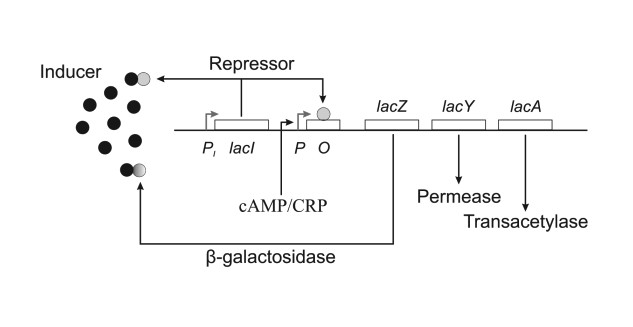
\includegraphics[width=0.8\linewidth]{lac.png}
	\caption{The \textit{lac} operon schematic}
	\label{fig:lac_operon}
\end{figure}

\section{Methodology}
Two experiments are carried out with detailed procedures explained in the handout \cite{goossens93}. Experiment 1 uses the $\Delta lacl$ strain of the bacteria (with lacl gene turned off), different inducers such as lactose, IPTG, glucose (and control) are used to investigate the behaviour of the \textit{lac} operon without the repressor. \\ \\
In the second experiment, three different strains of bacteria (wild type, $\Delta lacY$ and $\Delta lacIZY$) are investigated under different inducers (IPTG and lactose), the activity of $\beta$-glactosidase is measured at constant intervals (60 minutes to 150 minutes with 30 minutes intervals). \\ \\
The activity of $\beta$-glactosidase is quantified using the o-nitrophenyl-$\beta$-$D$-galactoside (ONPG) assay as described by Miller \cite{miller}. $OD_{600}$ is taken first to measure the bacterial cell density in the culture. The sample is then mixed was Z-buffer, SDS and chloroform, then vortexed for 10 seconds to lyse the cells. ONPG is then added and samples are incubated at 37 degrees Celsius for 20 minutes. $Na_2CO_3$ is then added to stop the reaction. All the samples are then left until the end when $OD_{420}$ and $OD_{550}$ readings are taken. $OD_{420}$ measures of the amount of o-nitrophenol which is the product of $\beta$-galactosidase catalyzed breakdown of ONPG thus it is a measure of $\beta$-galactosidase activity, $OD_{550}$ is measured to correct for cell debris. Finally $\beta$-glactosidase activity ($\beta A$) is calculated using the following equation (with the constant 1000 with unit mol/cell$\times$min$\times$ml which converts the activity per time, per volume, per cell density to molecules of enzyme per cell):
$$
\beta A = 1000 \dfrac{OD_{420}-1.75OD_{550}}{t\times V\times OD_{600}}
$$
In the equation above, $t$ is the incubation time for the assay in minutes (20 mins in this case), and $V$ is the volume in ml of the culture used in the assay (in this case, 0.2ml).
\section{Discussion of Feedback Mechanisms}
In the wild type (wt) \textit{lac} operon, there are four feedback mechanisms, two positive and two negative. The two positive feedbacks are:
\begin{enumerate}
  \item Active transport by lactose permease producing a higher concentration of $\beta$-galactosides and lactose inside the cell thereby increasing the expression of lacY which codes for lactose permease
  \item Transgalactosylation by $\beta$-galactosidase produces allolactose from lactose thereby increasing the expression of lacZ which codes for $\beta$-galactosidase
\end{enumerate}
The two negative feedbacks are:
\begin{enumerate}
  \item $\beta$-galactosidase hydrolyzes allolactose thereby decreasing the amount of inducer in the cell which reduces the amount of $\beta$-galactosidase
  \item $\beta$-galactosidase hydrolysis of lactose and allolactose also increases the glucose concentration in the cell which causes catabolite repression, making the transcription of \textit{lac} genes more difficult. This mechanism is bypassed if IPTG is used instead of lactose.
\end{enumerate}
In experiment 1, with the $\Delta lacl$ strain of the bacteria, without the repressor, $\beta$-galactosidase, permease and transacetylase are all constantly expressed, therefore there is no effects of positive feedback since transcription occurs at a constant rate. However the second type of negative feedback persists as the cyclic adenosine mono-phosphate (cAMP) site is still active and can still influence the binding difficulty of RNA polymerase.\\
In experiment 2, $\Delta lacY$ means no lactose permease is expressed which eliminates the first positive feedback mechanism; $\Delta laclZY$ eliminates all the feedback mechanisms.
\section{Analysis of Results}
\begin{figure}[htp]
\centering
\begin{subfigure}{.5\textwidth}
  \centering
  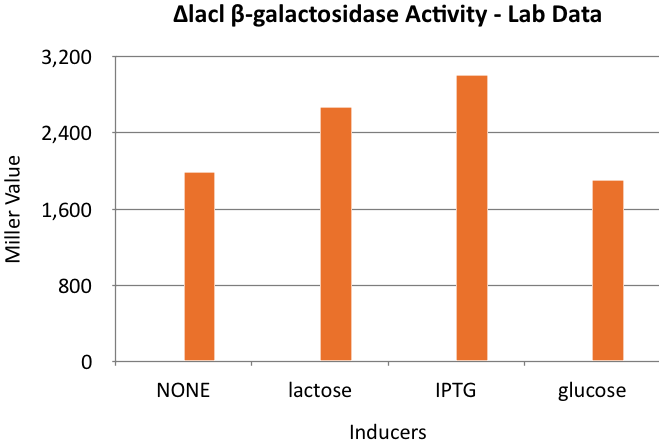
\includegraphics[width=1\linewidth]{lacl_lab.png}
	\caption{from lab}
	\label{fig:lacl_lab}
\end{subfigure}%
\begin{subfigure}{.5\textwidth}
  \centering
  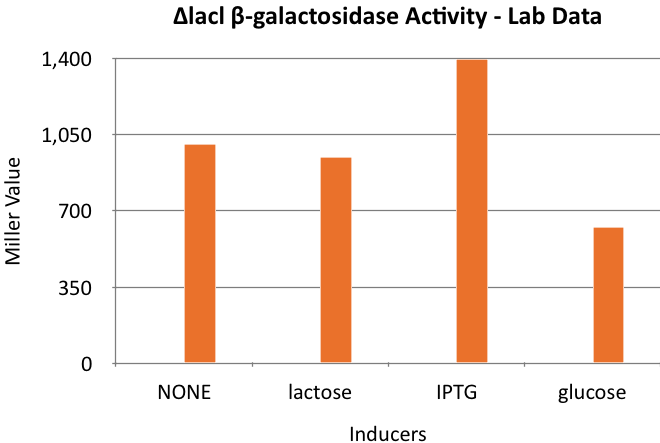
\includegraphics[width=1\linewidth]{lacl_exp.png}
  \caption{from example data}
  \label{fig:lacl_exp}
\end{subfigure}
\caption{$\Delta lacl$ beta-galactosidase activity}
\label{fig:lacl}
\end{figure}
Both the lab data and example data of experiment 1 is shown in figure \ref{fig:lacl}. With the strain of bacteria missing the supressor, $\beta$-galactosidase is constantly expressed. Therefore with the absence of any inducers there should still be $\beta$-galactosidase activity. This is confirmed in both the lab and experimental data. With lactose as an inducer, $\beta$-galactosidase breaks down lactose to glucose which decreases the cAMP level within the cell causing less of them to bind with the cAMP site. Therefore it is expected that less RNA polymerase binds to the promoter thereby decreasing the expression of $\beta$-galactosidase activity. This is shown in the example data but not the lab data, this may due to a number of errors within the experiment which is discussed in the conclusion. IPTG behaves in a similar way to allolactose and across both example and lab data there shows an increase in $\beta$-galactosidase activity, this behaviour is unaccounted for in our simple model of \textit{lac} operon described in section 1, as IPTG does not get broken down to glucose the expected behaviour is for the $\beta$-galactosidase activity to stay the same as the control with no inducers under the absence of the repressor, one possible explanation is that the $\Delta$lacl strain given may still be containing some wild-types and positive feedback within them dictates only a small amount of the strain present will produce large amount of $\beta$-galactosidase activity. With glucose as an inducer, the amount of cAMP within the cell decreases (more than using lactose as inducer), causing cAMP site to be on average less occupied thereby decreasing the transcription which results in a decrease in the activity of $\beta$-galactosidase, this behaviour is observed in both lab and example data.\\ \\
In experiment 2, $\beta$-galactosidase assay is carried out at varying time intervals thus the activity of different strains of bacteria under different inducers can be tracked, figure \ref{fig:all} shows the $\beta$-galactosidase activity for wild-type (wt), $\Delta$lacY and $\Delta$laclZY strains under both lactose and IPTG inducers, figure \ref{fig:all_lab} shows the lab data obtained and figure \ref{fig:all_exp} shows the example data obtained during previous sessions.\\ \\
Analyzing the result obtained on the wt strain of bacteria, it is expected that when lactose is used as the inducer, all four types of feedback mechanisms are present as lactose is broken down to allolactose which acts as the inducer for the repressor promoting positive feedback, and it is broken down into glucose which reduces cAMP level in the cell causing less transcription (negative feedback). It is also expected that there may be a time delay until activity in $\beta$-galactosidase is observed as there needs to be a basal level of $\beta$-galactosidase before the induction of the \textit{lac} operon. Initially there is positive feedback but also closely followed by negative feedback (dominated by the first type where $\beta$-galactosidase hydrolyzes the allolactose).
When IPTG is used as the inducer, as it does not get broken down into glucose but mimics the effect of allolactose, the effect of second type of negative feedback (cAMP level feedback) is eliminated which means the $\beta$-galactosidase level will still be rising over longer time period until other limiting factors are reached. Also it acts as the inducer straight away for the repressor which means the $\beta$-galactosidase activity is observed without any basal level (time delay). Thus it is expected for the graph of wt+IPTG to increase over time and for $wt$+lactose to increase after a time delay. This is confirmed largely through both the lab and the example data, some discrepancies such as the slight dip in activity at 150 minutes for wt+IPTG in \ref{fig:all_lab} all be accounted for through experimental error (see conclusion).\\ \\
Without the presence of lactose permease coded by the lacY gene, in the experiments with $\Delta$lacY, it is anticipated that there should be little discrepancies between $\Delta$lacY and wt type under IPTG as an inducer as it passes the cell membrane through active transport or diffusion, with lactose as the inducer however, under the $\Delta$lacY strain much less $\beta$-galactosidase activity should be observed as lactose has difficulty getting through the cell membrane, the little amount that gets through is quickly broken down into glucose without producing too much allolactose acting as the inducer that increases $\beta$-galactosidase activity. This is observed across both the lab and example data, again small discrepancies can be due to experimental error.\\ \\
Lastly, the $\Delta$lacIZY IPTG sample: this has the promoter deleted, along with the lacY required for lactose permease and importantly lacZ which encodes the hydrolysis enzyme, β-galactosidase. Thus, there will be no expression of the β-galactosidase and nearly zero activity which is shown in both the lab and example data.
\begin{figure}[htp]
\centering
\begin{subfigure}{.5\textwidth}
  \centering
  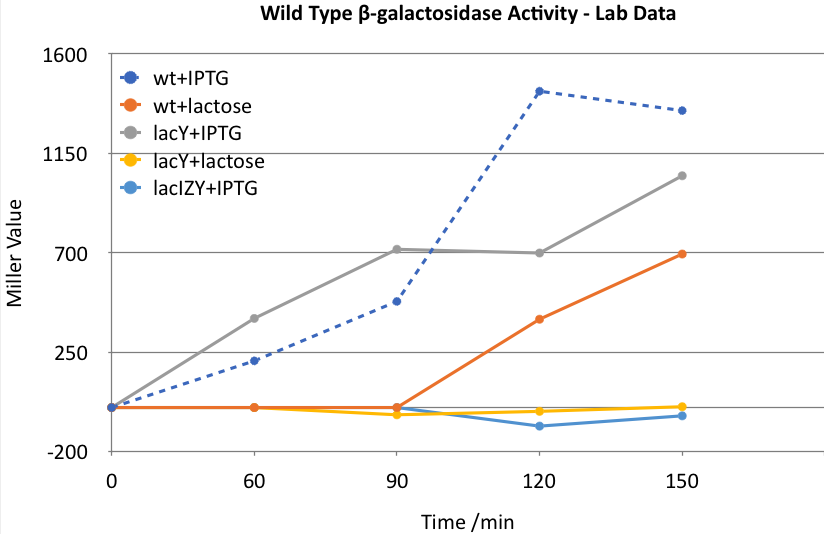
\includegraphics[width=1\linewidth]{all_lab.png}
	\caption{from lab}
	\label{fig:all_lab}
\end{subfigure}%
\begin{subfigure}{.5\textwidth}
  \centering
  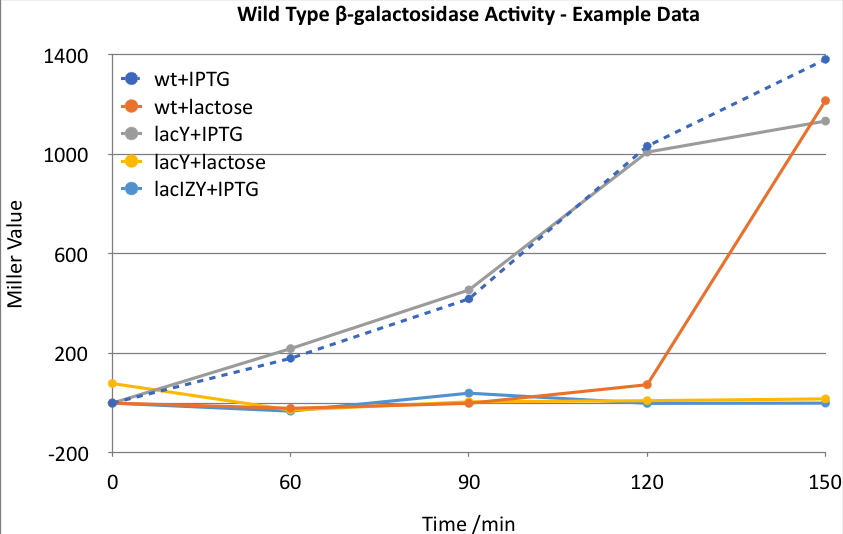
\includegraphics[width=1\linewidth]{all_exp.png}
  \caption{from example data}
  \label{fig:all_exp}
\end{subfigure}
\caption{wt, $\Delta lacY, \Delta lac$lYZ beta-galactosidase activity}
\label{fig:all}
\end{figure}
\section{Evaluation and Conclusion}
The experiments confirms the feedback mechanisms highlighted in section 3, the example data confirms all theory drawn from the simple model introduced in section 1, with the exception of increased $\beta$-galactosidase activity under $\Delta$lacl+IPTG. The minor discrepancies between the lab and example data could be due to a number of reasons:
\begin{enumerate}
  \item The spectrophotometer provided does not offer reliable result, i.e. consecutive readings yield different results
  \item As all experiments are conducted either simultaneously or within the same time window, their incubation time may differ from the actual incubation time for up to 30 minutes
  \item Inaccuracy in displacing solutions using pipettes across multiple samples
  \item Accidentally using the same pipette tips causing the mixing of different samples
  \item Chloroform discolours the cuvette causing inaccurate readings
  \item Incorrect/inconsistent amount of different solutions added to different samples
\end{enumerate}
These sources of errors can be mitigated through:
\begin{enumerate}
  \item Conducting different experiments at different time periods
  \item Use equipment (spectrophotometer) of higher quality which produces more repeatable results
  \item Be more proficient at conducting experiments like this and average readings over multiple experiments
\end{enumerate}
In conclusion, through the analysis and comparison of both the lab and example data to the simple model suggested, with an acceptable margin of error it is shown that the feedback mechanisms in the \textit{lac} operon follows the model highlighted in section 1.

\bibliographystyle{plainnat}
\bibliography{mytestbib}
\end{document}
